\chapter{Il progetto e il suo sviluppo}\label{chapter:formattazione}
%
\section{Tree Structure}\label{sec:cap_sec_subsec}

La tree structure~\ref{fig:treeStructure} del progetto si suddivide in diverse sottocartelle.\\ 
Di seguito, commenterò solo le cartelle che risultano rilevanti per la discussione:
\begin{itemize}
	\item \textbf{wwwroot}: Contiene file per la gestione della parte grafica, 
	in particolare, include, in apposite sottocartelle, i file HTML, CSS, JavaScript e le immagini utilizzate. 
	\item \textbf{Areas}: Contiene i file generati automaticamente dal framework ASP.NET Core Identity.
	\item \textbf{Controllers}: Contiene i file scritti in linguaggio C\# che svolgono un 
	ruolo fondamentale nella gestione delle richieste HTTP e nell'orchestrazione 
	delle azioni dell'applicazione.\ Questi file fungono da punto di ingresso per 
	le richieste HTTP, coordinano le azioni dell'applicazione, manipolano i dati e 
	restituiscono risposte HTTP appropriate.
	\item \textbf{Migrations}: Contiene i file in linguaggio C\# relativi alle migrations.
	\item \textbf{Models}: Contiene solo file C\#, che vengono utilizzati per rappresentare 
	le entità e i dati all'interno dell'applicazione, contribuendo così a mantenere il 
	codice organizzato e coeso.
	\item \textbf{Query}: Contiene esclusivamente file SQL, il cui utilizzo è ormai superato.\ 
	I file contenuti in questa cartella non influenzano l'esecuzione della piattaforma.\
	In particolare, questi file erano stati originariamente utilizzati per conservare le procedure, 
	ma sono state successivamente rimpiazzate dall'uso del framework Dapper. 
	\item \textbf{View}: Contiene numerosi file di tipo CSHTML, organizzati in diverse 
	sottocartelle.\ Questi file sono responsabili di come i dati vengono presentati 
	all'utente, gestendo l'aspetto, la struttura e l'interfaccia utente dell'applicazione.
\end{itemize}
%
\begin{figure}[ht]
	\centering
	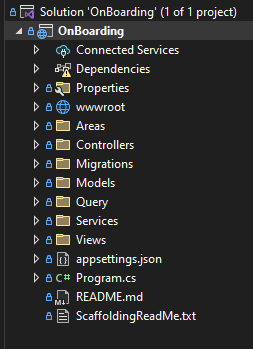
\includegraphics[width=0.4\textwidth]{img/treeStructure.png}
	\caption{tree structure del progetto}
	\label{fig:treeStructure}
\end{figure}
%
\section{Database}\label{sec:cap_sec_subsec}
Una parte sostanziale del lavoro impiegato per portare a compimento il
progetto si è concentrata in modo dettagliato sulla creazione del database,
ritenuto elemento cruciale per assicurare il pieno funzionamento della
piattaforma. 
\\ \\ 
La creazione del database è stata articolata in diverse fasi chiave:
\begin{itemize}
	\item Progettazione della struttura del database, un processo attentamente studiato.
	\item Scrittura del database in linguaggio SQL, una tappa essenziale per l'implementazione della struttura.
	\item Implementazione delle interrogazioni al database nella sezione di back-end,
	      facendo uso della libreria Dapper.
\end{itemize}
\textit{Nota}: il database è stato creato e gestito unicamente in locale per questioni di semplicità e per
l'esecuzione di test sulla correttezza della struttura e dell'implementazione del database stesso.
%
\subsection{Progettazione}
La fase di progettazione~\ref{fig:progettazione_database} del database ha occupato un ruolo
fondamentale nel corso di questo processo, coinvolgendo un'analisi costante e
una riflessione profonda. L'obbiettivo principale è stato quello di plasmare un
database estremamente completo, in grado di soddisfare appieno le esigenze
della piattaforma di e-learning, ponendosi lo scopo aggiuntivo di:
\begin{itemize}
	\item Migliorare la leggibilità del database;
	\item Rendere più agevole la manutenzione;
	\item Fornire ampie possibilità di estensione del sistema.
\end{itemize}
\begin{figure}[ht]
	\centering
	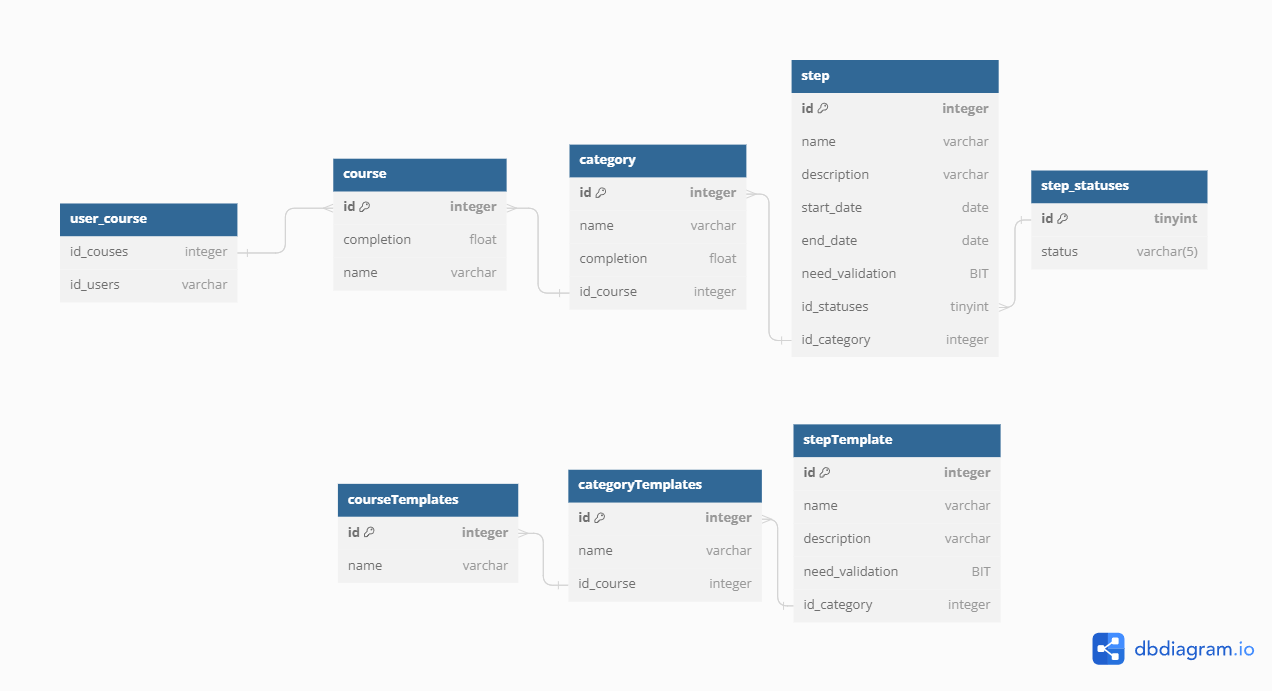
\includegraphics[width=1\textwidth]{img/progettazione_database.png}
	\caption{progettazione del database}
	\label{fig:progettazione_database}
\end{figure}
\textit{Nota}: la progettazione mostrata non tiene traccia delle tabelle utente, perchè vengono
gestite automaticamente dal progetto .NET grazie al servizio di autenticazione già
incluso (libreria \inlinecode{Microsoft.AspNet.Identity.EntityFramework;}).
%
\\ \\
Si noti, inoltre, che non è stato creato un collegamento tra le tabelle “*Templates” con il resto del tabelle
perchè esse vengono gestite in maniera del tutto indipendente con le altre informazioni e relazioni presenti.
\begin{figure}[ht]
	\centering
	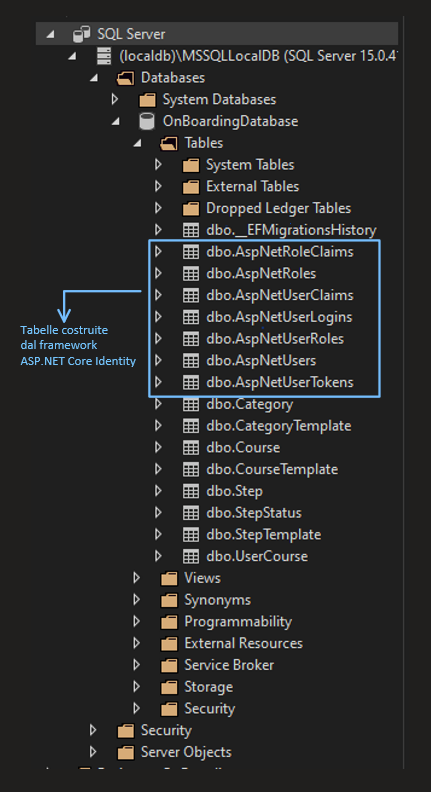
\includegraphics[width=0.5\textwidth]{img/TreeStructureDatabase.png}
	\caption{Tree structure del database}
	\label{fig:TreeStructureDatabase}
\end{figure}
%
\subsection{Scrittura nel linguaggio SQL}
Il risultato finale di questa fase è il seguente~\ref{appendice-database} (non sono riportate le tabelle
generate dal servizio di Autenticazione, perchè gestite automaticamente dalla
libreria a disposizione)
%
\subsection{Interrogazioni al Database}
Inizialmente, le interrogazioni al database erano state sviluppate attraverso
\href{https://learn.microsoft.com/it-it/sql/relational-databases/stored-procedures/stored-procedures-database-engine?view=sql-server-ver16}{stored
	procedure}.\ Tra i numerosi vantaggi proposti, l'idea principale era ottenere:
\begin{itemize}
	\item Riutilizzo del codice;
	\item Semplificazione della manutenzione;
	\item Prestazioni migliorate;
\end{itemize}
Tuttavia, durante lo sviluppo dell'applicativo, grazie al suggerimento di alcuni membri
dell'azienda, si è preferito sostituire le procedure con interrogazioni dirette dal codice
tramite il framework \href{https://learn.microsoft.com/it-it/azure/azure-sql/database/elastic-scale-working-with-dapper?view=azuresql}{Dapper}, al fine di poter migliorare:
\begin{itemize}
	\item Prestazioni in termini di tempo;
	\item Semplificare il debugging del codice;
	\item Centrallizzare l'intera logica in un unico posto.
\end{itemize}
All'interno della piattaforma si possono distinguere 3 macro categorie di interrogazioni per:
\begin{itemize}
	\item Inserimento dei dati riguardanti:
		\begin{itemize}
			\item utenti
			\item corsi;
			\item categorie (sotto gruppo dei corsi);
			\item step (sotto gruppo delle categorie);
			\item corsi template;
			\item categorie template (sotto gruppo dei corsi template);
			\item step template (sotto gruppo delle categorie template).
		\end{itemize}
	\item Eliminazione dei dati riguardanti:
		\begin{itemize}
			\item utenti
			\item corsi;
			\item categorie (sotto gruppo dei corsi);
			\item step (sotto gruppo delle categorie);
			\item corsi template;
			\item categorie template (sotto gruppo dei corsi template);
			\item step template (sotto gruppo delle categorie template).
		\end{itemize}
	\item Lettura dei dati per permettere di ottenere tutte le informazioni necessarie
		per la generazione corretta della pagina dinamica dato un determinato utente
		connesso;
\end{itemize}
%
\section{Scrittura del codice C\#}\label{sec:cap_sec_subsec}
La parte del codice back-end rappresenta il nucleo vitale dell'intero progetto, 
che ne garantisce il corretto funzionamento. Questa componente è stata completamente 
sviluppata utilizzando il linguaggio di programmazione C\#.
\\ \\
L'obbiettivo principale è stato garantire una gestione efficiente del database
direttamente attraverso il codice, sfruttando appieno le potenzialità del
framework Dapper. \\ 
Utilizzando C\# e il framework Dapper, è stato possibile
realizzare un corretto collegamento tra dati e utenti.\ Questo ha reso
possibile la generazione dinamica e accurata delle pagine web, consentendo
un'esperienza utente ottimale. 
\\ \\ 
Per eseguire delle query al database è
stato necessario creare una connessione dal codice C\# al database attraverso
la libreria \inlinecode{Microsoft.Data.SqlClient;}
%
%TODO: fixhere
\begin{lstlisting}[style=cs_style, caption=classe per ottenere la stringa di connessione per il collegamento al database]
using Microsoft.Data.SqlClient;
using Microsoft.EntityFrameworkCore;

namespace OnBoarding.Services
{
	public class ConnectionService
	private SqlConnection _connection = new SqlConnection();
	private SqlCommand _command = new SqlCommand();

	public static IConfiguration? Configuration { get; set; }

	public string GetconnectionString()
	{
		var builder = new ConfigurationBuilder().SetBasePath(Directory.GetCurrentDirectory()).AddJsonFile("appsettings.json");

		Configuration = builder.Build();
		return Configuration.GetConnectionString("ApplicationDBContextConnection");
	}


	public SqlConnection GetConnection() 
	{
		return _connection;
	}

	public SqlCommand GetCommand()
	{
		return _command;
	}

	}
}
\end{lstlisting}
%
In questo modo, una volta che è stata stabilita una connessione, 
è stato reso possibile il processo di scrittura di query. A titolo esemplificativo, si può menzionare 
la query nella funzione denominata ``GetCourses'' presente all'interno del file ``CourseManager.cs''.\ Questa query, 
quando viene fornito l'ID dell'utente come input, ha lo scopo principale di recuperare e restituire 
l'insieme completo dei corsi associati all'utente specificato.
%
%TODO: fixhere
\begin{lstlisting}[style=cs_style, caption=esempio funzione per l'esecuzione di una query da codice tramite il framework Dapper]
public List<CourseModel> GetCourses(string userid)
{
	using (_connection = new SqlConnection(connectionService.GetconnectionString()))
	{
		_connection.Open();

		string sql = 
			@"SELECT DISTINCT Course.* 
			FROM Course, AspNetUsers, UserCourse 
			WHERE UserCourse.UserId = @userId     
			AND UserCourse.CourseId = Course.Id";
		var coursesList = _connection.Query<CourseModel>(sql, new { userId = userid }).ToList();

		_connection.Close();

		return coursesList;
	}
} 
\end{lstlisting}
%
Si osserva che ciascun utente può essere associato a più corsi, 
stabilendo così una relazione uno a molti.\ Pertanto, è fondamentale 
che il valore restituito dalla funzione sia di tipo \inlinecode{List\textless CourseModel \textgreater}, 
in quanto questa struttura dati può contenere più di un corso associato a 
un utente specifico.\ Inoltre, grazie all'uso di Dapper, è possibile effettuare 
un'interrogazione al database mediante una stringa appositamente creata 
(come mostrato nelle righe 7\--11 del codice).\ Successivamente, è possibile 
ottenere il risultato dell'interrogazione corrispondente al parametro ``userid'' 
fornito alla funzione e al campo ``userId'' nella tabella ``Course'' (riga 12 del codice).
\\
Notare che siccome la funzione ritorna in questo caso una lista, il risultato della query
dovrà essere convertito in una collezione di oggetti dello stesso tipo (attraverso alla funzione \inlinecode{ToList()}).
%
\\ \\
%
Un punto di particolare rilevanza che merita menzione è rappresentato dallo sviluppo di una classe denominata 
``StatisticsController.cs''.\ Il suo scopo principale consiste nell'elaborare in modo esaustivo e dettagliato tutte 
le statistiche associate a un utente specifico.\ Questa classe si avvale della sofisticata libreria \inlinecode{ClosedXML.Excel;} 
per generare dati statistici in formato csv~\ref{fig:exportToExcel}, inerenti al completamento dei corsi che sono stati non solo avviati, ma anche portati a 
termine dall'utente in questione.\ È essenziale sottolineare che questa funzionalità è rigorosamente riservata agli 
utenti che detengono il privilegiato ruolo di ``Admin''.
%
% TODO: fix position
\begin{figure}[ht]
	\centering
	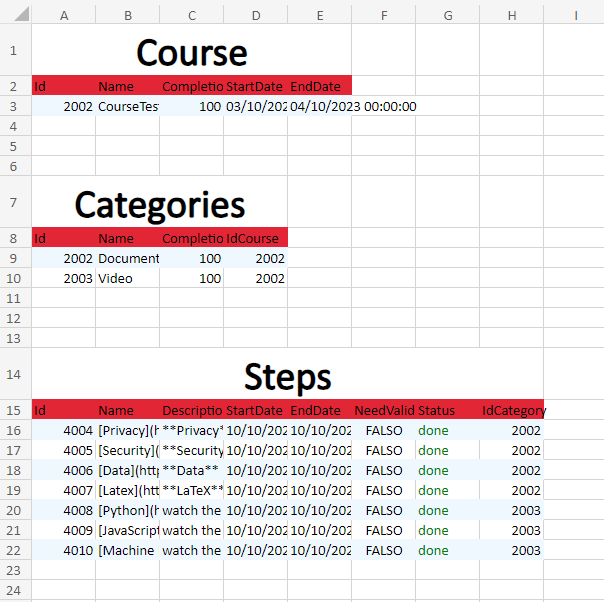
\includegraphics[width=0.7\textwidth]{img/exportToExcel.png}
	\caption{esempio di conversione in csv}
	\label{fig:exportToExcel}
\end{figure}
%
\begin{lstlisting}[style=cs_style, caption=funzione utilizzata per l'esportazione in file exel]
[HttpGet]
[Authorize(Roles = "Admin")]
public IActionResult ExportToExcel(int id)
{
	using (var workbook = new XLWorkbook())
	{
		CourseModel course = _courseManager.GetCourseByID(id);

		var ws = workbook.Worksheets.Add(course.Name); // Sheet Name
		int i = 1;

		/////////////////////////////////////// Course
		ws.Range($"A{i}:E{i}").Merge();
		ws.Cell(i, 1).Value = "Course";
		ws.Cell(i, 1).Style.Font.Bold = true;
		ws.Cell(i, 1).Style.Alignment.Horizontal = XLAlignmentHorizontalValues.Center;
		ws.Cell(i, 1).Style.Font.FontSize = 30;

		// Header
		i++;
		ws.Cell(i, 1).Value = "Id";
		ws.Cell(i, 2).Value = "Name";
		ws.Cell(i, 3).Value = "Completion";
		ws.Cell(i, 4).Value = "StartDate";
		ws.Cell(i, 5).Value = "EndDate";
		ws.Range($"A{i}:E{i}").Style.Fill.BackgroundColor = XLColor.Alizarin;

		// Body
		i++;
		ws.Cell(i, 1).Value = course.Id;
		ws.Cell(i, 2).Value = course.Name;
		ws.Cell(i, 3).Value = course.Completion;
		if (course.StartDate != DateTime.MinValue) ws.Cell(i, 4).Value = course.StartDate.ToString();
		else { ws.Cell(i, 4).Value = "NULL"; ws.Cell(i, 4).Style.Font.FontColor = XLColor.Red; }
		if (course.EndDate != DateTime.MinValue) ws.Cell(i, 5).Value = course.EndDate.ToString();
		else { ws.Cell(i, 5).Value = "NULL"; ws.Cell(i, 5).Style.Font.FontColor = XLColor.Red; }
		ws.Range($"A{i}:E{i}").Style.Fill.BackgroundColor = XLColor.AliceBlue;
		i += 1;

		// ...
		// Stesso procedimento appena descritto per i Corsi, viene fatto
		// per le Categorie e gli Step 
		
		using (var stream = new MemoryStream())
		{
			workbook.SaveAs(stream);
			var content = stream.ToArray();
			return File(
					content,
					"application/vnd.openxmlformats-officedocument-spreadsheetml.sheet",
					course.Name + ".csv"
				);
		}
	}
}
\end{lstlisting}
%
Un aspetto di notevole rilevanza è stato il processo di gestione dei dati statistici all'interno della pagina denominata 
``/Views/Statistics/Index.cshtml''.\ Questa pagina ha una funzione fondamentale poiché consente agli admin di visualizzare 
l'insieme completo delle statistiche.\ Ciò è reso possibile grazie alla capacità di ordinare agevolmente le informazioni 
presenti all'interno delle tabelle.\ Questa caratteristica permette agli utenti di organizzare i dati in base alle loro 
specifiche esigenze e criteri di ricerca.
\\
Inoltre, per rendere l'esperienza ancora più interattiva e informativa, è stata inclusa una sezione di codice dedicata 
direttamente all'interno della pagina stessa, utilizzando il tag \inlinecode{\textless\ script \textgreater\ \dots \textless\ /script \textgreater}. Questo approccio ha 
consentito di incorporare efficacemente dei grafici che offrono una rappresentazione visiva dei dati statistici.\ 
Questi grafici sono stati sviluppati in modo da offrire quattro diverse visualizzazioni, ognuna delle quali fornisce un'analisi 
dettagliata dei dati statistici, permettendo agli utenti di comprendere meglio i pattern e le tendenze sottostanti.
\begin{itemize}
	\item due grafici a barre;
	\begin{itemize}
		\item Il primo rappresenta la somma totale dei corsi suddivisi per stato di completamento (done, running, todo);
		\item Il secondo rappresenta il numero di corsi completati in relazione al mese dell'anno.
	\end{itemize}
	\item due grafici a torta;
	\begin{itemize}
		\item Il primo rappresenta il tempo medio di completamento necessario per terminare uno specifico corso, suddiviso per corso;
		\item Il secondo rappresenta il tempo medio di completamento necessario per teminare uno specifico corso, suddiviso per utenti.
	\end{itemize}
\end{itemize}
L'implementazione del codice per la creazione dei grafici è stata effettuata mediante l'uso del linguaggio di programmazione JavaScript.\ 
Un aspetto interessante da sottolineare è che i dati numerici necessari per la creazione dei grafici non sono stati ottenuti direttamente 
tramite il codice JavaScript, ma sono stati acquisiti attraverso apposite funzioni getter scritte in codice C\#.\ 
Questo approccio è stato adottato per garantire l'accuratezza e la coerenza dei dati, nonché per sfruttare le funzionalità di gestione 
dei dati messe a disposizione dal linguaggio C\#.\
In sostanza, il processo è stato il seguente: il codice JavaScript si è interfacciato con il codice C\# attraverso apposite funzioni getter, 
ottenendo così i dati numerici necessari per alimentare i grafici.\
\begin{lstlisting}[style=javascript_style, caption=esempio sezione codice Javascript per la creazione di un grafico a barre per la rappresentazione dei dati]
<script>
	// ...
	
	// -------------------------------- BAR CHART
    var xValues = ["To Do", "Running", "Done"];
    var yValues = [@todo, @running, @done, 0];
    var barColors = ["red", "#e5e600", "green"];

    new Chart("BarChart", {
        type: "bar",
        data: {
            labels: xValues,
            datasets: [{
                backgroundColor: barColors,
                data: yValues
            }]
        },
        options: {
            legend: { display: false },
            title: {
                display: false,
                text: ""
            }
        }
    });

	// ...
</script>
\end{lstlisting}
%
\begin{figure}[ht]
	\centering
	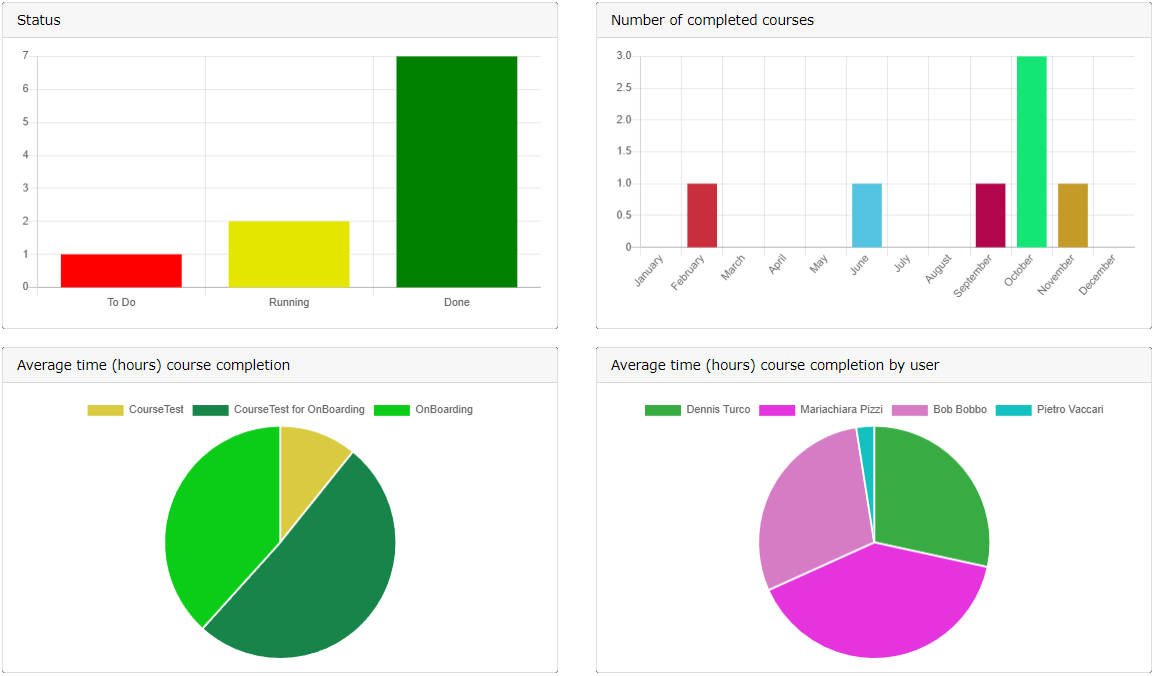
\includegraphics[width=0.7\textwidth]{img/charts.png}
	\caption{grafici per la visualizzazione dei dati}
	\label{fig:charts}
\end{figure}
%
\section{Layout della piattaforma}\label{sec:cap_sec_subsec}
Nonostante alcune limitazioni evidenti nel design della piattaforma, che potrebbe essere descritto come non completamente moderno e, 
in alcuni aspetti, forse un po' troppo minimalista, il layout della piattaforma è stato progettato e realizzato con l'obiettivo di 
creare un servizio che sia estremamente intuitivo e facile da utilizzare, sia per gli utenti 
che per gli amministratori responsabili della gestione degli accessi e del progresso degli utenti 
durante il loro percorso nell'esperienza.\ Grazie a questa attenzione all'usabilità, 
è stato possibile assicurarsi che l'intera esperienza sia accessibile e fruibile in modo agevole 
e soddisfacente per tutti i suoi utilizzatori.
\\ \\
%TODO: aggiungere l'info di quali linguaggi ho utilizzato per l'aggiunta di questa specifica integrazione
% e magari mostrare la parte di codice se rilevante
Un'aggiunta di notevole interesse dal punto di vista del layout è stata l'integrazione 
della visualizzazione in sintassi Markdown.\ Questa nuova funzionalità mira a migliorare 
l'esperienza dell'utente durante la visualizzazione delle descrizioni delle informazioni 
testuali presenti all'interno dei corsi.\ L'obiettivo è ottenere una visualizzazione che 
favorisca una maggiore leggibilità delle informazioni e permetta l'integrazione di 
elementi come immagini, titoli, sottotitoli e molto altro all'interno delle descrizioni 
dei task.\ Questo offre maggiore flessibilità e personalizzazione agli amministratori 
incaricati della creazione dei corsi.
%TODO: fixhere
\begin{figure}[ht]
	\centering
	\begin{subfigure}{0.3\textwidth}
		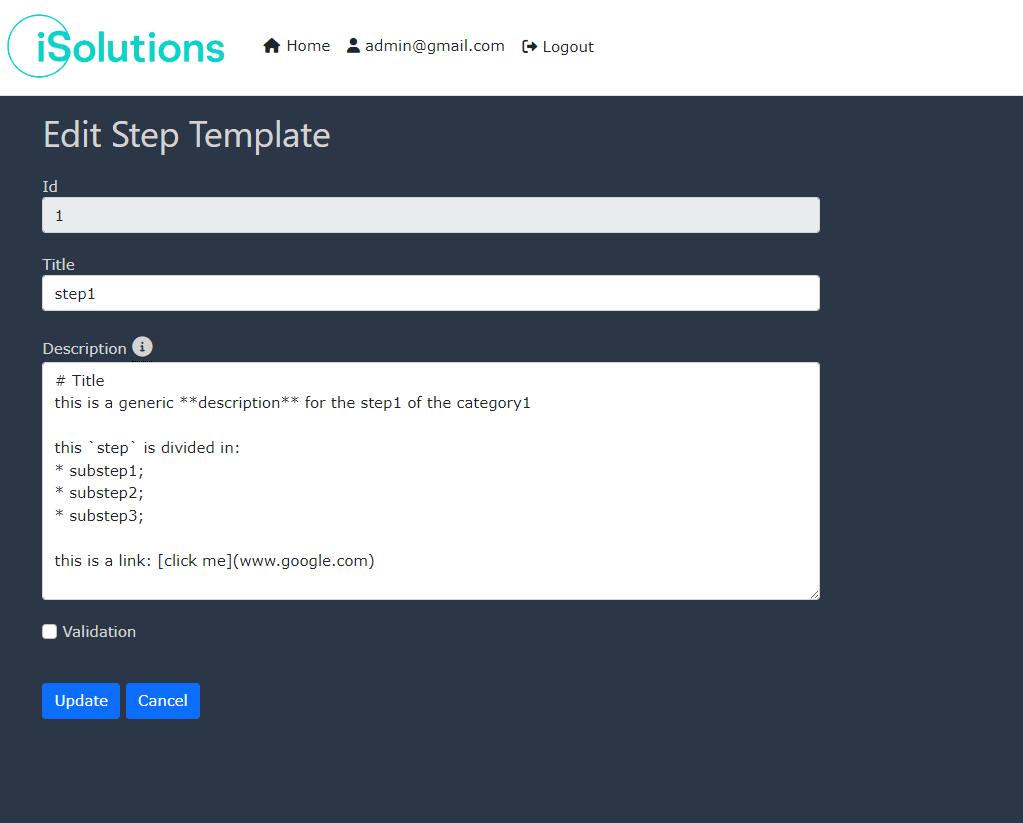
\includegraphics[width=1.4\textwidth]{img/markdown_p1.png}
		\caption{scrittura in Markdown}
	\end{subfigure}%
	\begin{subfigure}{0.3\textwidth}
		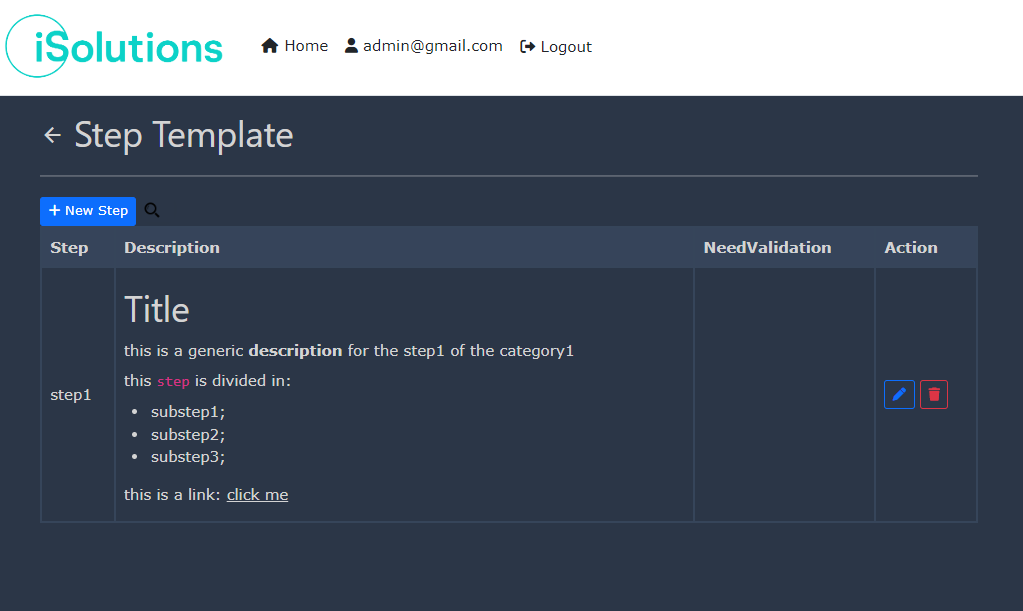
\includegraphics[width=1.4\textwidth]{img/markdown_pt2.png}
		\caption{visualizzazione in Markdown}
	\end{subfigure}
	\caption{esempio di scrittura e visualizzazione in Markdown}
	\label{fig:markdown}
\end{figure}
%
\\
Inoltre, per agevolare l'utilizzo di questa funzionalità, è stato incluso un apposito 
messaggio pop-up~\ref{fig:markdownGuide} che fornisce una semplice guida all'uso, completa di esempi pratici, 
al fine di consentire agli utenti di sfruttarla al meglio.
\begin{figure}[ht]
	\centering
	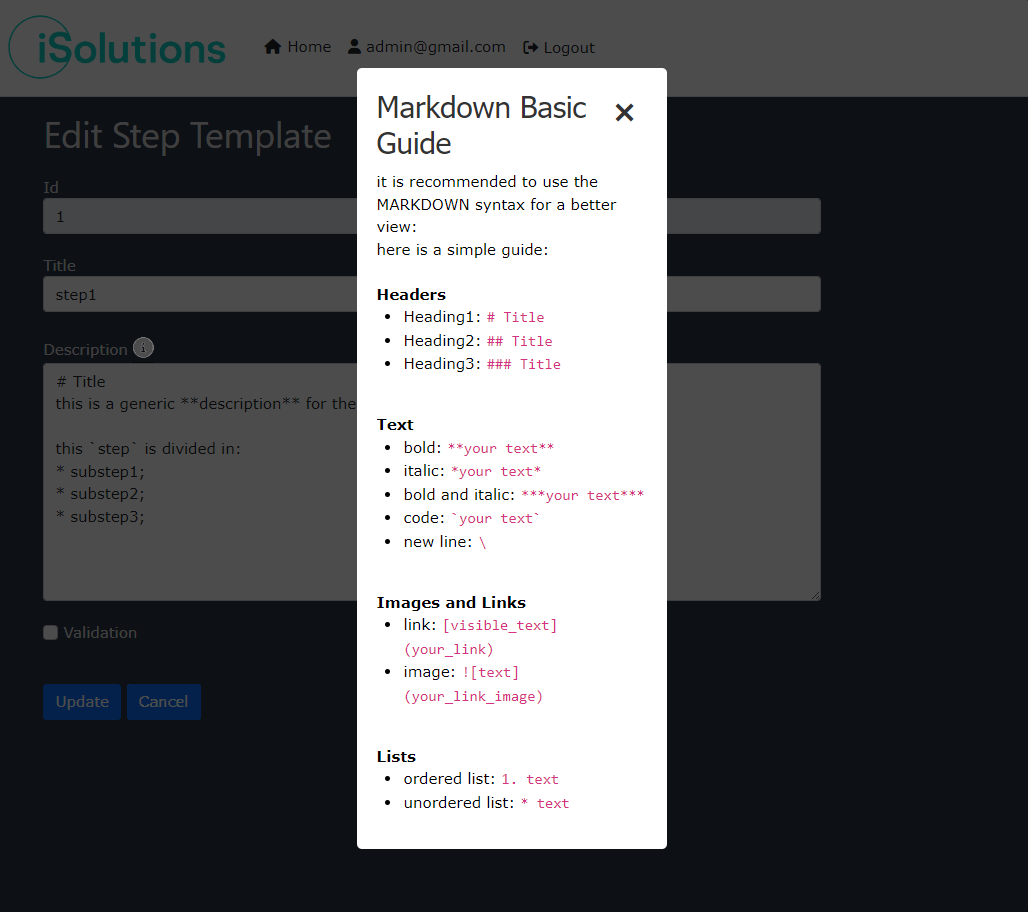
\includegraphics[width=0.7\textwidth]{img/markdownGuide.png}
	\caption{Guida basilare al Markdown}
	\label{fig:markdownGuide}
\end{figure}